\section*{The Rules}

In order to study mathematical plays and answer the many questions they raise, a new mathematical field of study was developed and many new terms were created. The phrase ``mathematical play" is in itself a new term, for instance. While the most common term is "Combinatorial Games", the canonical reference for this field \textit{Winning Ways for Your Mathematical Plays} 1981, uses the former, not the latter. As more is said about the topic, more meaning the term ``mathematical play" is going to acquire.

The name ``Combinatorial Game" might bring to light some information. It, at least, means that this field will deal with games, as in, an instance of a Game Theory problem, and, more specifically, a subset of those games. It also brings to light that the use of counting, finite structures and, most likely, graph representations are omnipresent. However, a definition of the object of interest becomes possible with the name mathematical play.

To play something mathematically could be understood as to engage in an activity in which the better use of mathematical ability, such as counting and logic, would result in advantage over its poor use. However it could be detailed further to an activity in which mathematical ability is the single defining factor. The later might make more sense because there are games, like poker, that do require some counting ability. However, luck and reading behavior skills are much more valuable to a successful game and this is something the definition would be better off forbidding.

\defi{Chance moves}, like throwing a dice or flipping a card, are not fit for mathematical plays. Even with their removal, however, there are possibilities that would not be comfortably called mathematical plays. The nature of a mathematical plays is that both players can engage the same activity and generate advantages out of ``good play". For instance, it would be hard to agree that two people playing rock-paper-scissors are battling a mathematical fight, even though there are no chance moves.

It is very important that all players have \defi{complete information} of the position. Games like rock-paper-scissors, in which players take action simultaneously, block complete information. Therefore, players must \textbf{move alternately}. The last concerning factor in discerning mathematical from non-mathematical plays during this analysis is the number of players.

When each player has more than one opponent a goal greater than gaining advantage arises. When playing with over two people it is frequent that the best move is not the one that brings a better position but one that prevents any of the opponents from gaining an winning advantage. While that can be very mathematical, there is a clear distinction between sticking to two player games and allowing any number of players. Notice that one can consider soccer as a two player game - even though there are multiple agents in a team. In order to focus on the mathematical ability to make the best move, the option to allow only \textbf{two players} is the most interesting.

The only remaining criteria of this definition, as established in [\todo{WW}], is related to the term play, and not the term mathematical. The rules of the game must guarantee that from any starting position, \defi{\todo{play should always} end because a player will not have moves available}. If following ``\defi{normal play}" convention, a player that cannot move is lost. It is  correct to assume normal play, unless specified otherwise, in this field of study.

The foundations of mathematical plays, highlighted, give light to a complex and rich set of problems, although, at the same time, other complex and rich problems are left behind. The game of chess, for example, does not meet the ending condition and, therefore, is left out. Fortunately, games like chess might benefit from these studies with adaptations or additional rules (although they do not consist of good examples of combinatorial games).\\
Let us consider the following game:\\

\begin{figure} [!ht]
\begin{center}
	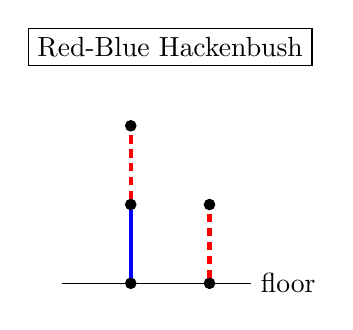
\begin{tikzpicture}
	\node[draw] (title) at (1.5, 3) {Red-Blue Hackenbush};
	\node (p1) at (0,0) {};
	\node (p2) at (3,0) {floor};
	\begin{scope} [every node/.style={scale=0.4, circle, draw, fill=black}]
	\node (p3) at (1,0) {};
	\node (p4) at (1,1) {};
	\node (p5) at (1,2) {};
	\node (p6) at (2,0) {};
	\node (p7) at (2,1) {};
	\draw (p1) -- (p2);
	\begin{scope} [ultra thick]
	\draw[blue] (p3) -- (p4);
	\draw[red, densely dashed] (p4) -- (p5);
	\draw[red, densely dashed] (p6) -- (p7);
	\end{scope}
	\end{scope}
	\end{tikzpicture}
\end{center}
\caption{}
\end{figure}

In RB-Hackenbush, a move is made by taking a single colored edge of the image and removing any edges that become disconnected from the floor. The player called \textbf{Left} can only remove \textbf{bLue and soLid}, edges, and the other, called \textbf{Right}, \textbf{Red and dashED} edges. It is a common practice to assume that all games are played between Left (blue) and Right (red), although, occasionally, new colors will be presented. In this text, every color also has a matching style.

The RB-Hackenbush is a game by the routine definitions of game, meaning it has a clear ruleset and potential to be fun. It is also a game by the definition above, which will be the new ``routine" one used going forward. However, the instance of this game drawn above is also called a game. In the future, when analyzing a board state for example, the word position may seem to make more sense, but the correct word is game. The meaning of the word must be deduced from context.

The \textbf{game tree} term refers to the routine meaning, for example. The image below is the game tree that arises from the game, instance, presented above.

\begin{figure} [H]
\begin{tikzpicture}
[
	sibling distance=150pt,
	level distance=100pt,
	level 1/.style={sibling distance=6cm},
	level 2/.style={sibling distance=3cm},
	every node/.style = {
			shape=rectangle,
			rounded corners,
			draw,
			align=center,
			top color=white,
			bottom color=blue!20
		},
	every child/.style = {
		ultra thick
	}
]
\node[] (title) at (0, 3) {Game Tree};
\coordinate (p1) at (0.5,0);
\coordinate (p2) at (2.5,0) {};
\node {
	\begin{tikzpicture}
	[
		every node/.style = {
			scale=0.4,
			circle,
			draw,
			fill=black
		},
		ultra thick
	]
			\node (p3) at (1,0) {};
			\node (p4) at (1,1) {};
			\node (p5) at (1,2) {};
			\node (p6) at (2,0) {};
			\node (p7) at (2,1) {};
			\draw (p1) -- (p2);
			\draw[blue] (p3) -- (p4);
			\draw[red, densely dashed] (p4) -- (p5);
			\draw[red, densely dashed] (p6) -- (p7);
	\end{tikzpicture}
}
child [draw=blue] {
	node [thin, black] {
	\begin{tikzpicture}
	[	
		every node/.style = {
			scale=0.4,
			circle,
			draw,
			fill=black
		},
		ultra thick
	]
	\node (p6) at (2,0) {};
	\node (p7) at (2,1) {};
	\draw (p1) -- (p2);
	\draw[red, densely dashed] (p6) -- (p7);
	\end{tikzpicture}} 
	child [draw=red, dashed] {node [thin, solid, black] {} } }
	child [draw=red, dashed] {node [thin, solid, black] {
		\begin{tikzpicture}
		[	
		every node/.style = {
			scale=0.4,
			circle,
			draw,
			fill=black
		},
		ultra thick
		]
		\node (p3) at (1,0) {};
		\node (p4) at (1,1) {};
		\node (p5) at (1,2) {};
		\draw (p1) -- (p2);
		\draw[blue] (p3) -- (p4);
		\draw[red, densely dashed] (p4) -- (p5);
		\end{tikzpicture}
}
	child [draw=blue, solid] {node [thin, black] {} }
	child [draw=red, dashed] {node [thin, solid, black] {
			\begin{tikzpicture}
			[	
			every node/.style = {
				scale=0.4,
				circle,
				draw,
				fill=black
			},
			ultra thick
			]
			\node (p3) at (1,0) {};
			\node (p4) at (1,1) {};
			\draw (p1) -- (p2);
			\draw[blue] (p3) -- (p4);
			\end{tikzpicture}
	}
	child [draw=blue, solid] {node [thin, black] {} }
	}
}
child [draw=red, dashed] {node [thin, solid, black] {
		\begin{tikzpicture}
		[	
		every node/.style = {
			scale=0.4,
			circle,
			draw,
			fill=black
		},
		ultra thick
		]
		\node (p3) at (1,0) {};
		\node (p4) at (1,1) {};
		\node (p6) at (2,0) {};
		\node (p7) at (2,1) {};
		\draw (p1) -- (p2);
		\draw[blue] (p3) -- (p4);
		\draw[red, densely dashed] (p6) -- (p7);
		\end{tikzpicture}
} 
	child [draw=blue, solid] {node [thin, solid, black] {
			\begin{tikzpicture}
			[	
			every node/.style = {
				scale=0.4,
				circle,
				draw,
				fill=black
			},
			ultra thick
			]
			\node (p6) at (2,0) {};
			\node (p7) at (2,1) {};
			\draw (p1) -- (p2);
			\draw[red, densely dashed] (p6) -- (p7);
			\end{tikzpicture}
}
child [draw=red, dashed] {node [thin, solid, black] {} } }
	child [draw=red, dashed] {node [thin, solid, black] {
			\begin{tikzpicture}
			[	
			every node/.style = {
				scale=0.4,
				circle,
				draw,
				fill=black
			},
			ultra thick
			]
			\node (p3) at (1,0) {};
			\node (p4) at (1,1) {};
			\draw (p1) -- (p2);
			\draw[blue] (p3) -- (p4);
			\end{tikzpicture}
}
	child [draw=blue, solid] {node [thin, black] {} } }};
\end{tikzpicture}
\caption{Method used to build a game tree}
\end{figure}



In the tree above the styled edges, in the same pattern as before, between configurations tells which player made a move. The game trees used in \todo{CGT} may me slightly different
as they, from each configuration, develop the moves from both players. This is a most import characteristic because it allows the sum of trees.

As noted previously, the game tree contains all the information required in order to calculate the number, or non-number, a game is equal to. The Surreal Numbers \todo{KNUTH} have a recursive nature that can be completely separated from games. However, as they were created analyzing a position like the one above \todo{ONAG}, its definition will be presented in terms of moves.

The model Conway, Berlekamp and Guy created to analyze games is based on finding the advantage a player has over the other. The calculation, in this model, of this advantage is given in terms of spare moves. For now, the reader may found this weird because the advantage might actually rely on the ability of the players, but when analyzing games it is important to expect both players play perfectly. Since a player loses if he or she cannot move, counting spare moves is counting how many sequential moves a player can make before reaching \defi{equity} in the position.

Equity is found in \defi{zero positions}. Zero position are those in which the first player to move loses. The idea to call such positions zero made sense for Conway, and, therefore, in his new set of numbers, if a game \Gm is in a zero position, \Gm{=0}. If left \textbf{can win} regardless of who starts, we call it positive, and, in the other way around, negative. In more special positions, a hint on the topic of this text, in which the first to play can win, we call them fuzzy.

\begin{figure} [H]
	\begin{center}
		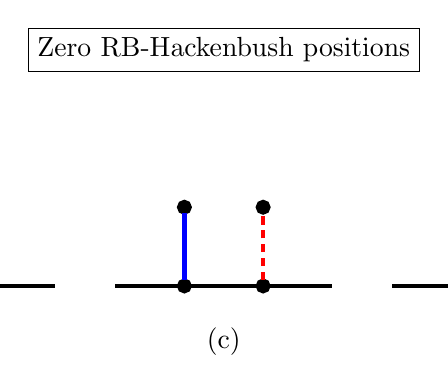
\begin{tikzpicture}
			\node[draw] (title) at (1.5, 3) {Zero RB-Hackenbush positions};
			\node (p1) at (0,0) {};
			\node (p2) at (3,0) {};
			\begin{scope} [ultra thick, every node/.style={scale=0.4, circle, draw, fill=black}]
				\node (p3) at (1,0) {};
				\node (p4) at (1,1) {};
				\node (p6) at (2,0) {};
				\node (p7) at (2,1) {};
				\draw (p1) -- (p2);
				\draw[blue] (p3) -- (p4);
				\draw[red, densely dashed] (p6) -- (p7);
			\end{scope}
			\coordinate[thick, label=(c)] () at (1.5, -1);
			\hspace{-200pt}{ \begin{scope} [ultra thick, every node/.style={scale=0.4, circle, draw, fill=black}]
				\draw (p1) -- (p2);
			\end{scope}}
			\coordinate[thick, label=(a)] () at (1.5, -1);
			\hspace{100pt}{ \begin{scope} [ultra thick, every node/.style={scale=0.4, circle, draw, fill=black}]
				\node (p3) at (1,0) {};
				\node (p4) at (1,1) {};
				\node (p5) at (1,2) {};
				\node (p6) at (1.5,0) {};
				\node (p7) at (1.5,1) {};
				\node (p8) at (2, 0) {};
				\node (p9) at (2, 1) {};
				\draw (p1) -- (p2);
				\draw[blue] (p3) -- (p4);
				\draw[blue] (p4) -- (p5);
				\draw[red, densely dashed] (p6) -- (p7);
				\draw[red, densely dashed] (p8) -- (p9);
			\end{scope}}
			\coordinate[thick, label=(b)] () at (1.5, -1);
			\hspace{200pt}{ \begin{scope} [ultra thick, every node/.style={scale=0.4, circle, draw, fill=black}]
				\node (p3) at (1,0) {};
				\node (p4) at (1,1) {};
				\node (p5) at (1,2) {};
				\node (p6) at (2,0) {};
				\node (p7) at (2,1) {};
				\node (p8) at (2,2) {};
				\draw (p1) -- (p2);
				\draw[blue] (p3) -- (p4);
				\draw[red, densely dashed] (p4) -- (p5);
				\draw[red, densely dashed] (p6) -- (p7);
				\draw[blue] (p7) -- (p8);
			\end{scope}}
			\coordinate[thick, label=(d)] () at (1.5, -1);
			\hspace{100pt}{ \begin{scope} [ultra thick, every node/.style={scale=0.4, circle, draw, fill=black}]
				\node (p3) at (1,0) {};
				\node (p4) at (1,1) {};
				\node (p6) at (2,0) {};
				\node (p7) at (2,1) {};
				\node (p8) at (1.5,2) {};
				\draw (p1) -- (p2);
				\draw[blue] (p3) -- (p4);
				\draw[red, densely dashed] (p4) -- (p8);
				\draw[red, densely dashed] (p6) -- (p7);
				\draw[blue] (p7) -- (p8);
			\end{scope}}
			\coordinate[thick, label=(e)] () at (1.5, -1);
		\end{tikzpicture}
	\end{center}
	\caption{Several instances of 0 positions in RB-Hackenbush}
\end{figure}

Although all games have the same value, the games are not the same. The  way to represent a game derives from its game tree. The game is composed of two sets of games and $\mid$ is used as delimiter. The game (a) is one where neither player has available moves and, because of that, the game $(a) = 0 = \gam{0}{0}$. (c), on the other had, is \gam{\gam{}{\gam{}{}}}{\gam{\gam{}{}}{}}, that simplifies to \gam{\gam{}{0}}{\gam{0}{}}. The games that form each of left and right sets are the configurations reachable by left and right, in a recursive definition.

The notations is exactly the same for numbers, but they should not be confused. For a game  \Gm{= \{x_1, \ldots, x_n \mid y_1, \ldots, y_m\}} to be a number, it must be true that:
$$\forall x_i \in X, \forall y_j \in Y, x_i < y_j$$

The process of finding the number a game is equal to is the theme of the next section. With that said, some new number already showed up in the figure above. The number \{ 0 $\mid$ \}, for example. What would be a pleasant real number for it? 1, because in this game, left has exactly one move to spare.

For the next few concepts a new game must be presented as RB-Hackenbush is incapable of generating fuzzy positions. However, a proof that all such games are numbers is due, and will be provided in the next section.

\begin{figure} [!ht]
	\begin{center}
		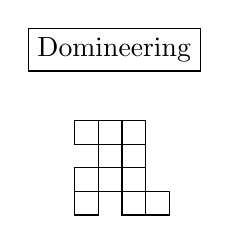
\begin{tikzpicture}
		\node[draw] (title) at (0.5, 1.8) {Domineering};
		\draw[] (0.6,-0.3) rectangle ++(0.3,0.3);
		\draw[] (0.9,-0.3) rectangle ++(0.3,0.3);
		\draw[] (0,-0.3) rectangle ++(0.3,0.3);
		\draw[] (0,0) rectangle ++(0.3,0.3);
		\draw[] (0.3,0) rectangle ++(0.3,0.3);
		\draw[] (0.6,0) rectangle ++(0.3,0.3);
		\draw[] (0.3,0.3) rectangle ++(0.3,0.3);
		\draw[] (0.6,0.3) rectangle ++(0.3,0.3);
		\draw[] (0,0.6) rectangle ++(0.3,0.3);
		\draw[] (0.3,0.6) rectangle ++(0.3,0.3);
		\draw[] (0.6,0.6) rectangle ++(0.3,0.3);
		\end{tikzpicture}
	\end{center}
	\caption{}
\end{figure}

Domineering is played by placing, or marking, a 2x1 rectangle on the board, or drawing. Left plays in the vertical and right in the horizontal. The reader is invited to play the position above a few times, and realize that the player starting it is always able to win. In fact, with perfect play, both players can win with a move to spare. The quest for calculating the advantage a player has, so far, can be been summarized by the question: ``Who is ahead, by how much?". However, in positions such as the one above, a new question is more important: ``How big is the next move". \todo{Berlekamp 1}.

This second question is answered in temperature theory. Temperature theory must follow a detailed explanation and clear understanding of numbers and games, and, therefore, a good explanation will only take place in section 4. However, as this is the main tool used to develop the topic of this text, an idea will follow.

Temperature measures the activity of the position. The activity can be understood as the importance of the next moves. In chess, for example, closed positions would be colder than endgames positions. In the position below, being the next player to move is not that important. Both players would start improving the position of the pieces until one find a break-through. Being a move behind means less piece development but the game will progress slowly, reducing the impact of that.

\begin{center}
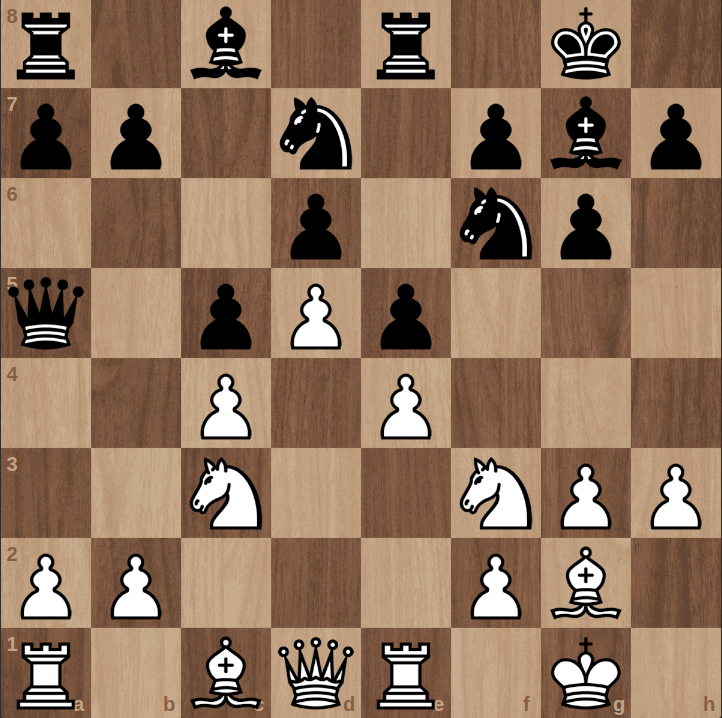
\includegraphics[scale=0.15]{images/chess_cold} 
\end{center}

In \textbf{hot} positions, opposed to \textbf{cold} position, the next moves are paramount for \textbf{both} players. In the board below, the player who moves first has a clear path to victory. It might be time to re-iterate that chess in itself is not a combinatorial game, although the following position can be considered one, as there are no drawing chances. In this specific position an subset of chess that removes stalemate from the ruleset is equivalent to chess, so it is possible to make it fit the definition.

\begin{center}
	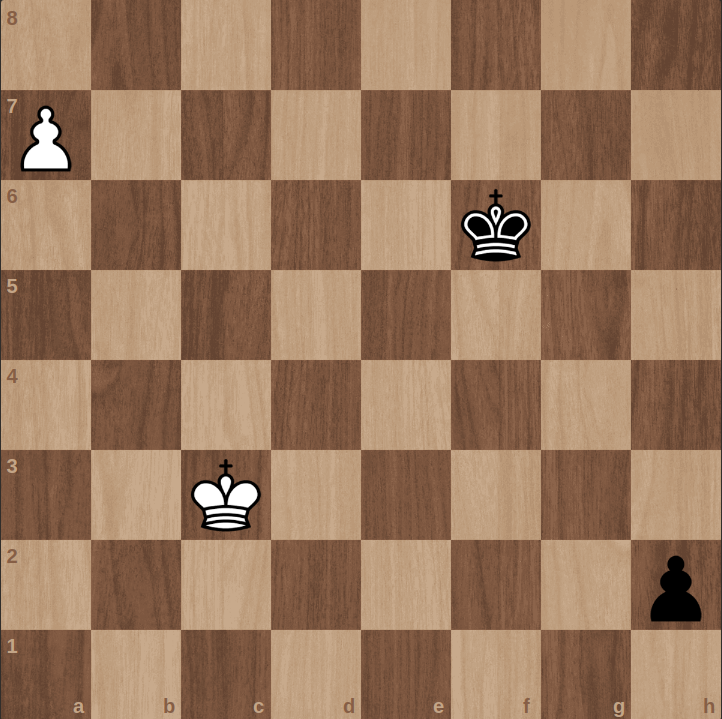
\includegraphics[scale=0.15]{images/chess_hot} 
\end{center}

It is correct to imagine that when putting a hot game \Gm{} in the notation \Gm{= \gam{X}{Y}}, then, $\exists x_i, y_j \mid x_i \ge y_j$, making it obvious that \Gm{} is not a number. On the closed position, the game might be cooler, but it will definitely heat up after a few moves. The endgame position above however, is becoming a number after the next move. Because it is becoming a number, it receives the special name \defi{switch}.

Switches are the most basic non-numbers. A switch is a non-numbers \Gm{} that both left's and right's best moves are numbers, but $G^L \ge G^R$. It is extremely easy to find the \defi{temperature} and \defi{bias} of such games. 

\begin{figure} [!ht]
	\begin{center}
		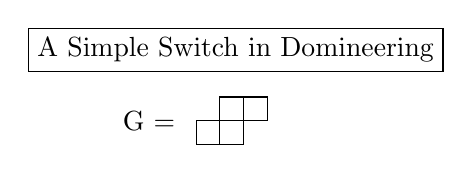
\begin{tikzpicture}
			\node[draw] (title) at (0.5, 0.9) {A Simple Switch in Domineering};
			\node (title) at (-0.6, 0) {G = };
			\draw[] (0.3,-0.3) rectangle ++(0.3,0.3);
			\draw[] (0.3, 0) rectangle ++(0.3,0.3);
			\draw[] (0.6, 0) rectangle ++(0.3,0.3);
			\draw[] (0,-0.3) rectangle ++(0.3,0.3);
		\end{tikzpicture}
	\end{center}
	\caption{}
\end{figure}

In this game left has a move that leads to a zero position and right has two moves that lead to the same game with value -1. Therefore, \Gm{= \gam{0}{{-}1}}. The bias is the average of $G^L, G^R$ that is equal to -0.5 in this case. The temperature is how much the game differs from the bias that is 0.5 in this case. A better way of writing this switch is $G = -0.5 \pm 0.5$. In general, a switch $H = \{x| y\}$ can be written as $H = (x+y)/2 \pm (x-y)/2$.

Calculating these values for general non-numbers is not simple enough to be completely conveyed at this point; Not because it is too hard or that describing it does not fit in the introductory pages, but because better understanding of numbers and arithmetic is required.






